%************************************************
\chapter{Draft}\label{ch:draft}
%************************************************


% TODO
% From Idemix To P2ABCE: reasons

\section{Smart card APDU}

To communicate the smart cards and the reader an standardized protocol is specified in ISO/IEC 7816-4 \citep{APDUISO}.

The messages, also kown as \ac{APDU}, are divided in APDU Commands and APDU Responses.

\textbf{APDU Commands} consist in 4 mandatory bytes (CLA, INS, P1, P2), and an optional payload.

\begin{itemize}
	\item CLA byte: Instruction class. Denotes if the command is interindustry standard or proprietary.
	\item INS byte: Instruction code. Indicates the specific command.
	\item P1, P2 bytes: Instruction parameters.
	\item Lc, 0-3 bytes: Command data length.
	\item Command data: Lc bytes of data.
	\item Le, 0-3 bytes: Expected response data length.
\end{itemize}

This way, minimal number of bytes are needed to transmit commands to the smart card, allowing manufacturer's personalization of the smart card behavior and capabilities along with standard operations.

\begin{figure}[bth]
	\begin{center}
		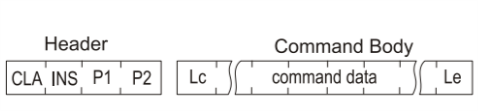
\includegraphics[width=0.55\linewidth]{gfx/APDUCommand}
	\end{center}
	\caption{APDU Command}
	\label{fig:APDUCommand}
\end{figure}


\textbf{APDU Responses} are generated inside the smart card, always as an answer to an APDU Command. They consist on an optional payload and two mandatory status bytes.


\begin{itemize}
	\item Response data: At most Le bytes of data.
	\item SW1-SW2 bytes: Status bytes. Encode the exit status of the instruction.
\end{itemize}

\begin{figure}[bth]
	\begin{center}
		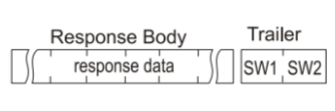
\includegraphics[width=0.55\linewidth]{gfx/APDUResponse}
	\end{center}
	\caption{APDU Response}
	\label{fig:APDUResponse}
\end{figure}




\hfil


The transmission protocol varies between different types of readers and smart cards (e.g. chip, contact-less), but what is common between every smart card interaction, is the \textit{APDU Command-Response Dialogue}. As long as the smart card has a power supply, it can maintain the dynamic memory in RAM between APDU Commands, what allows to do in two or more commmands complex operations, transmit more bytes than a single APDU can admit, etc.

\hfil




\begin{figure}[bth]
	\begin{center}
		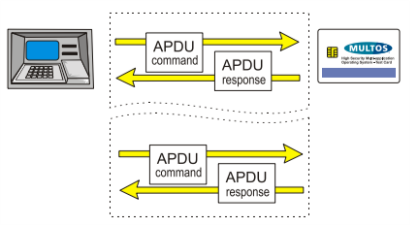
\includegraphics[width=0.75\linewidth]{gfx/APDUdialog}
	\end{center}
	\caption{APDU Command-Response Dialogue}
	\label{fig:APDUdialog}
\end{figure}

Originally, the Lc and Le bytes had only 1 byte if present, restricting the payload data to be at most 256 bytes long. An extension to the protocol changed the meaning of a Lc or Le 0x00 byte (256 bytes long payload), so when the byte corresponding to Lc or Le started with 0x00, the next two bytes where the real length.  With this, an Extended APDU lets up to 65536 bytes of data.

The problem here is that not all readers or smart cards support extended APDUs. Originally, to send more than 256 bytes of data, a new APDU Command instruction was defined so the smart card stored the payload in a buffer, until other APDU Command made use of it. To send more data in an APDU Response, the status bytes were set to: SW1=0x61 and SW2 to the remaining bytes to send. Because a smart card can't send APDU Commands, the card terminal then sends a GET RESPONSE, a special APDU Command, with Le set to the number of bytes specified in SW2. Iterating this process, the smart card could send as many bytes as it wanted.






\section{P2ABCE}


In the \ac{P2ABCE} repository \citep{p2abcurl} is available the project's code, divided in two solutions: a complete P2ABCE implementation in Java and a Multos Smartcard implementation as companion for the project.

The Java code is managed by a Maven project, structured using various known design patterns, but not of our interest. The structure we are actually interested in are the REST Services and their use of the Components classes, in which the smartcards are included.

P2ABCE project is based on the concept of smartcards to store the credentials, logical or physical. An interface is defined to communicate with these smartcards, and then different implementations allow to use either \textit{Software Smartcards} or \textit{Hardware Smartcards}. 

The \textit{SoftwareSmartcard} class implements the interface in Java, suitable for tests and self-stored smartcards that any application using P2ABCE may need.

The \textit{HardwareSmartcard} class uses the standard APDU messages [TODO:ref] to interact with smartcards. P2ABCE defines for every method in the mentioned interface, the necessary APDU instructions, and currently relies on \textit{javax.smartcardio} abstract classes (implemented by Oracle in their JRE) to communicate with the smartcard reader. This way, it doesn't matter what manufacturer issues the smartcard, or if it's an Android device, if they support the APDU API, P2ABCE will work with them.

\begin{figure}[bth]
	\begin{center}
		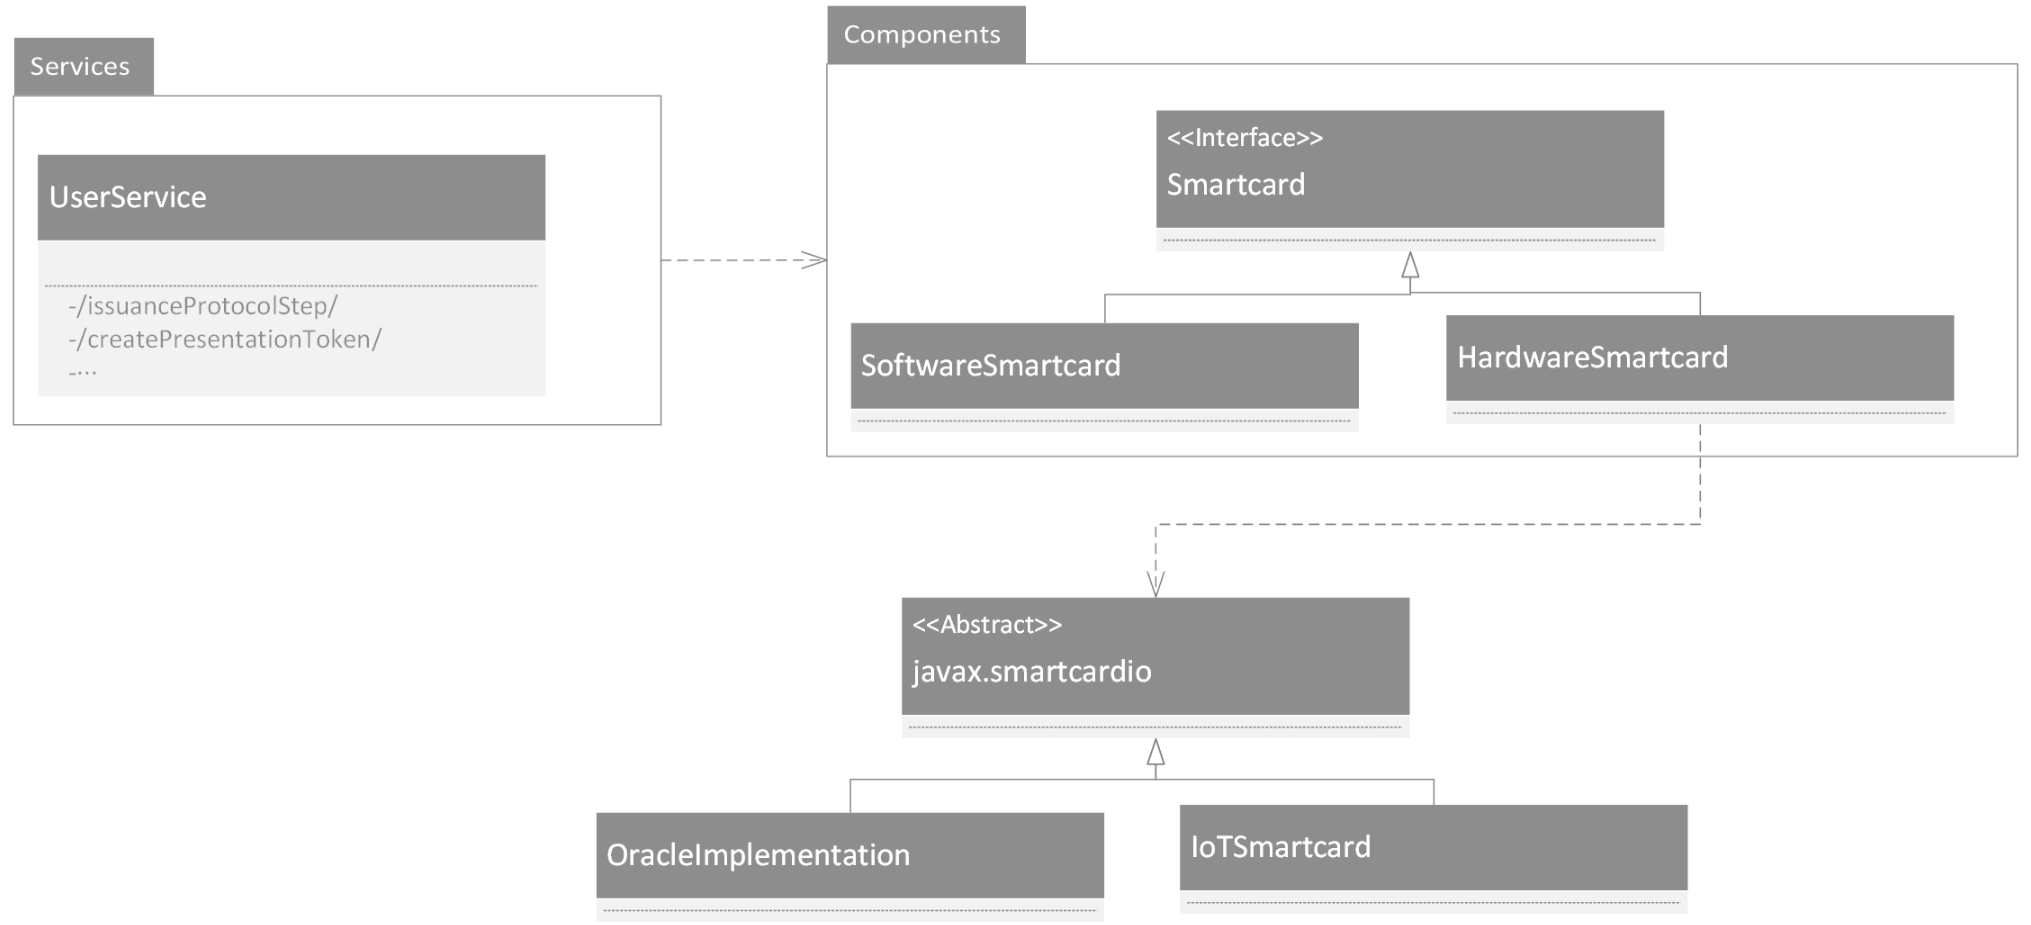
\includegraphics[width=\linewidth]{gfx/p2abceBasicUML}
	\end{center}
	\caption{Basic P2ABCE structure}
	\label{fig:p2abceBasicUML}
\end{figure}


As a PoC the P2ABCE project includes the ABC4Trust Card Lite, an implementation for ML3-36K-R1 Multos Smartcards. The code is written in C, but is very dependent on the Multos framework, aside from numerous bugs and bad coding habits. 



At this stage, we have two options to implement our IoT device compatible with P2ABCE:

\begin{itemize}
	\item Implement in C the \textit{Smartcard} interface used by P2ABCE architecture, and use some communication protocol to remotelly call the methods from the machine running the P2ABC Engine.
	\item Present the IoT device as a hardware smart card, using the APDU protocol (already defined, standard and with minimal overload). Providing a \textit{javax.smartcardio} ``IoT implementation'' to communicate with the IoT device through a transmission protocol, the already existing \textit{HardwareSmartcard} class can work with the new \textit{IoTSmartcard} in the IoT device.
\end{itemize}



%TODO : hablar más de los servicios REST



\section{MULTOS}

MULTOS is a multi-application smart card operative system, which provides a custom developing environment, with rich documentation \citep{MultosTechLib}. MULTOS smart cards communicate like any other smart card following the standard, but internally offers a very specific architecture, affecting the way one must code applications for it.

In this section we will present the main characteristics of a MULTOS smart card that shaped the ABC4Trust Card Lite code and that we had to be aware of when adapting it to IoT devices.

\paragraph{MULTOS programming languages} A native assembly language called MEL, C and, to a lesser extent, Java, are the available languages to code for MULTOS. In our case, ABC4T Card Lite uses MEL and C.

\paragraph{MULTOS Workflow}

Most of the transmission and communication process is done by MULTOS core, and it then selects, based on the CLA byte of the APDU, the application to load. This application is what most developers will only worry about, and is where their $main()$ function will start.

\begin{figure}[bth]
	\begin{center}
		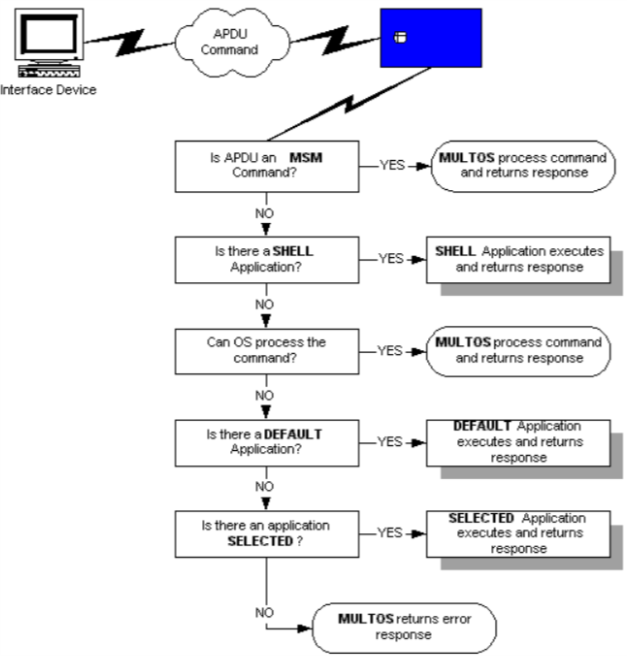
\includegraphics[width=\linewidth]{gfx/multosWorkflow}
	\end{center}
	\caption{MULTOS workflow}
	\label{fig:multosWorkflow}
\end{figure}

The application uses then the \textit{multos.h} file that declares multiple global variables already loaded with the needed data, including the APDU Command bytes.

Now the developer is in charge of checking what instruction was sent and if the APDU has the expected ISO Case. If everything is ok, code what needs to be run and write in specific data space the APDU Response bytes, call \textit{multosExit()} and MULTOS will be in charge to send the APDU Response.

In summary, our application starts with all data loaded and exits without worrying how to send the answer. A very comfortable workflow that we must now implement for our IoT device if we would want ABC4T Card Lite code to work.

\paragraph{MULTOS Memory Layout}

Each application in MULTOS has access to a specific memory layout, divided in different categories:

\begin{figure}[bth]
	\begin{center}
		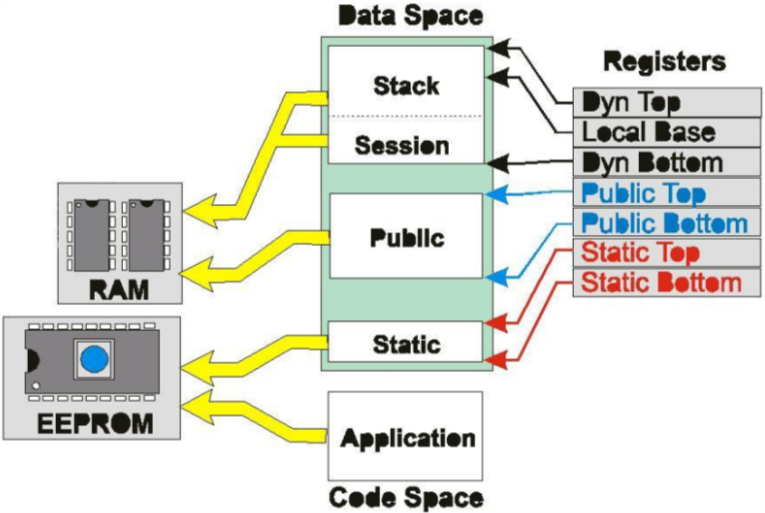
\includegraphics[width=\linewidth]{gfx/multosMemLay}
	\end{center}
	\caption{MULTOS Memory Layout}
	\label{fig:multosMemLay}
\end{figure}


The Code Space is where the application code is stored.
The Data Space is divided in Static memory, Public memory and Dynamic memory.

\textbf{Static memory} are the application variables declared after the specific \textit{\#pragma melstatic} compiler directive. These variables are stored in the non-volatile EEPROM, and any write is assured to be saved because they are not loaded into RAM.

\textbf{Public memory} can be seen as the input/output buffer for applications and MULTOS system. The APDU header appears at the top of Public, and command data at the bottom. The application writes then the APDU Response bytes in Public, at specific position (see \autoref{fig:multosPubMem}). To declare variables in this data space, the \textit{\#pragma melpublic} directive is available.

\textbf{Dynamic memory} works like usual program memory, with Session Data storing global variables and the Stack. The limited size of RAM in IoT devices and smart cards makes the use of dynamic memory not advisable. The compiler directive to use Session Data is \textit{\#pragma melsession}.


\begin{figure}[bth]
	\begin{center}
		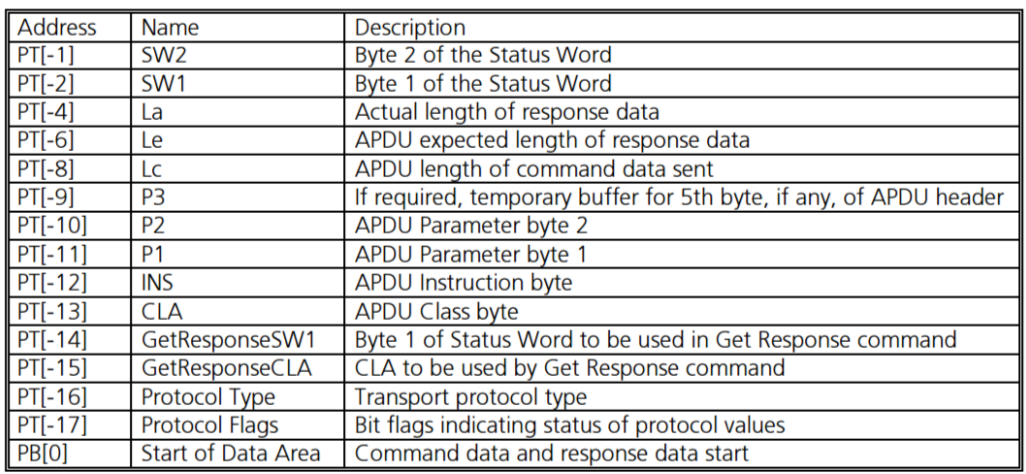
\includegraphics[width=\linewidth]{gfx/multosPubMem}
	\end{center}
	\caption{MULTOS Public Memory Data Map}
	\label{fig:multosPubMem}
\end{figure}


\hfil


With regards to primitive types, to avoid confusion with their sizes, MULTOS defines and uses the following data types specified in \autoref{fig:multosDataTypes}. It's important to notice that MULTOS is Big Endian
\marginpar{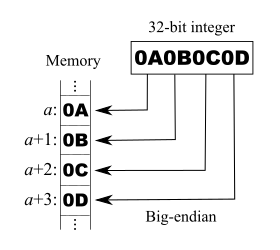
\includegraphics[width=\linewidth]{gfx/Big-Endian}\\Big-Endian, Wikipedia}
and when storing structures there is no padding between defined variables, unlike modern compilers that perform data structure alignment \citep{dataStructAlign} for performance.

\begin{figure}[bth]
	\begin{center}
		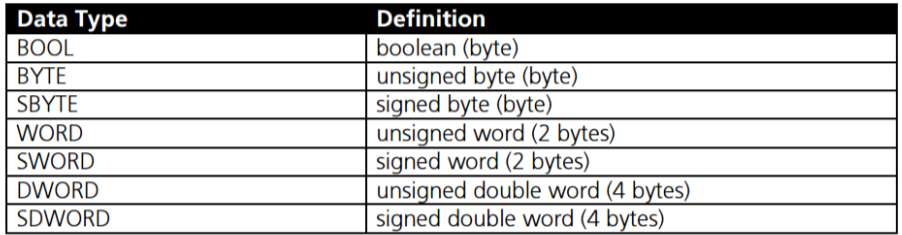
\includegraphics[width=\linewidth]{gfx/multosDataTypes}
	\end{center}
	\caption{MULTOS Data Types}
	\label{fig:multosDataTypes}
\end{figure}


\paragraph{MULTOS Standard C-API}

A collection of more than a hundred functions are provided for arithmetic, cryptography, memory and smart card operations. The \textit{multos.h} interface provides access to these functions, that ultimately call their respective primitive instructions in assembly code. The primitive instructions are but a system call with an operation code, loading data in the needed registers. Therefore,  no implementation for these tools is available, nor in C, nor in assembly code.

Nevertheless, the C-API documentation \citep{MultosTechLib} provides rich description for each function.





\section{ABC4Trust Card Lite}

P2ABCE provides a smart card reference implementation, ABC4Trust Card Lite \citep{ABC4TCardLite}. It supports device-bound U-Prove and Idemix, and virtually any discrete logarithm based pABC system.

Version 1.2 is based on MULTOS ML3 cards, with approximately 64KB of EEPROM (non-volatile memory), 1KB of RAM and an Infineon SLE 78 microcontroller, a 16-bit based CPU aimed for chip cards.

The card stores the user's private key $x$ and any \ac{BLOB} that the P2ABCE may need (like user's credentials). Then P2ABCE delegates the cryptographic operations on the smart card, that operates with $x$.

\begin{figure}[bth]
	\begin{center}
		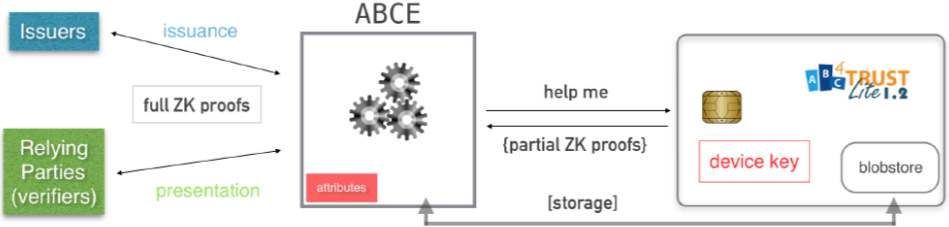
\includegraphics[width=\linewidth]{gfx/ABC4TCardLite}
	\end{center}
	\caption{ABC4Trust Card Lite}
	\label{fig:ABC4TCardLite}
\end{figure}

The cryptographic operations performed by the smartcard are the modular exponentiation and addition that discrete logarithm ZKPs are based on.

\hfil

The code is available from the P2ABCE project and has some good and bad points to have in count:

The best asset of this code is that it's written in C aiming to a very constrained device, similar in computational power to many IoT devices, and very limited memory.
	
Some \textit{tricks} in the code include using \textit{union} data types for variables that will be stored on the same data location, but at different moments (e.g. depending on APDU Command INS byte), minimizing this way the use of RAM and making code readability better; or strong use of pointers and \textit{memcpy} calls to copy structures with multiple variables as arrays of bytes.


Among the many drawbacks, we could highlight the awful coding, the strong dependency on MULTOS framework and some bugs found. 

The code is structured in two files, \textit{main.h} and \textit{main.c}, with 557 and 5157 lines of code respectively.

The file \textit{main.h} is mostly a reimplementation in assembly MEL of some MULTOS functionality already offered with latest \textit{multos.h}.

The \textit{main.c} consists on near 600 lines of variables and data structures declarations, followed by the \textit{main()} function, a 2635 lines long \textit{switch-case} with practically no comments, and to conclude, the implementation of thirty functions called \textit{Subroutines} at the end of the file.


This gives an idea of the problematic to maintain or even understand the code. But once one studies MULTOS framework in deep and applies many refactoring techniques to ABC4T Card's code, this becomes the best starting point for the IoT version.





\section{IoT and P2ABCE}

In this section we will define how an IoT device will be integrated in the P2ABCE environment, being totally compatible with any other system using P2ABCE, addressing the power and memory constrains IoT devices face.


\hfil

Our main goal is to make an IoT device capable to act as an User or Verifier in the P2ABCE architecture. For this, the device should manage complex XML schemas, perform cryptographic ZKP operations and communicate with the Verifier or Prover with which it's interacting.

The communication is already solved by the \textit{Internet} capabilities of IoT devices.

Our concern are the data artifacts exchanged as XML and the cryptographic operations involving secret keys that must remain private to the IoT device.

Here is where we look at the P2ABCE architecture more closely, and the concept of smart cards shows a solution for the second issue. Even in the case we were to implement all P2ABCE inside an IoT device, we would have to implement support for software smart cards, to keep the secret inside the IoT device. We will start building the house from the ground, implementing the smart card operations inside the IoT device.

Now that in our design we have the smart card, we need to address the first point, XML squemas. We understand with \textit{XML squemas} both managing the XML syntax and the whole process to generate a proper answer, that is, basically, the crypto engine that relies on Idemix and the smart card to hold the secret information.

Taking in consideration Idemix is currently provided in Java as a considerably big project, and version 3.0.36 still hasn't got official documentation, the task to port the Idemix crypto engine to IoT could be done in the future, if the chosen devices have enough storage and capacity. And even in that case, we would need to implement P2ABCE User and Verifier's architecture to completely free ourselves from an external P2ABCE machine.

The final port would be so big, many IoT devices would fall out of the requisites to run it, failing in our initial objective.

\hfil

After this analysis of the P2ABCE, we conclude that the mandatory requisite for any IoT device that wants to work with this system and keep its private keys in it, is to implement the smart card functionality, and delegate the rest of the operations on a machine capable of running P2ABCE, until that functionality is implemented for the IoT device. 


\hfil

This architecture is not really such an original idea. For example, IPv6 involves managing 128 bits per address and large headers, and many use cases only need IoT devices to communicate inside a private network. That's why many of them use 6LoWPAN to compress packets or use smaller address sizes. To communicate a 6LoWPAN with the Internet, a proxy is needed to transform 6LoWPAN packets to IPv6.

\hfil


Therefore, the IoT device now has a \textbf{duality} in its functions, because it is the User that starts any interaction with other systems, and it's also the smart card that P2ABCE delegates for crypto operations. It can also be seen as a \textbf{double delegation}. The IoT device delegates on the external P2ABCE server to manage the protocol, and the P2ABCE server delegates on the IoT, acting now as a smart card, for the cryptography.




\hfil

We find here two challenges: how to delegate from the IoT device to the P2ABCE delegation server, and how to transmit them and the APDUs to the IoT device.

Currently P2ABCE offers various REST web services to run different roles in P2ABCE system: User Service, Issuer Service, Verification Service, etc. An application that integrates P2ABCE can make use of this services in the same machine or implement the functionality using the core components written in Java, the same ones the REST services use. Our PoC machine, the Omega2, can make REST calls easily, but other devices may use \ac{CoAP}, and in that case, the P2ABCE REST services should be rewritten to offer CoAP support. The commands needed to delegate to the P2ABCE delegation server will be the same to operate with the REST services. This way, the first issue is solved.

The transmission of the messages will depend on the specific use case, capabilities and resources available. If the delegation server is connected, for example, through RS-232 serial with the IoT device, and physically inaccessible, in the same way an IoT device on its own would be protected, the communication is simple, and not far away from the Arduino Yun idea of combining two devices, one more powerful but to use only when needed. But if the IoT device and the delegation server are apart, or more than one IoT device delegates to it, then the transmission must be secured. They could use 6LoWPAN to talk to each other (the delegation service could be deployed in the proxy) and then secure communications with existing solutions, like with pre-shared symmetric keys, certificates for authentication and authorization, etc., it depends on each particular deployment.

At the end of the day, this is all about usual security in IoT. Many other studies focus on this matter, so we will assume it can be done, and will focus on what's new, P2ABCE in IoT.


\hfil


% TODO: imagen con servicios desplegados/actores en cada máquina


To sum up, our IoT device will act as User (Prover or Verifier) keeping its secrets in a software smart card. When it starts an interaction with other actor of the P2ABCE system (Issuer, Verifier, etc.), the IoT device will delegate with a remote call (using REST in our PoC) to a P2ABCE delegation server, attaching the XML file and the necessary information for the server to send the APDUs to the software smart card (in our PoC using TCP sockets, giving the IP and listening port).



\begin{figure}[bth]
	\begin{center}
		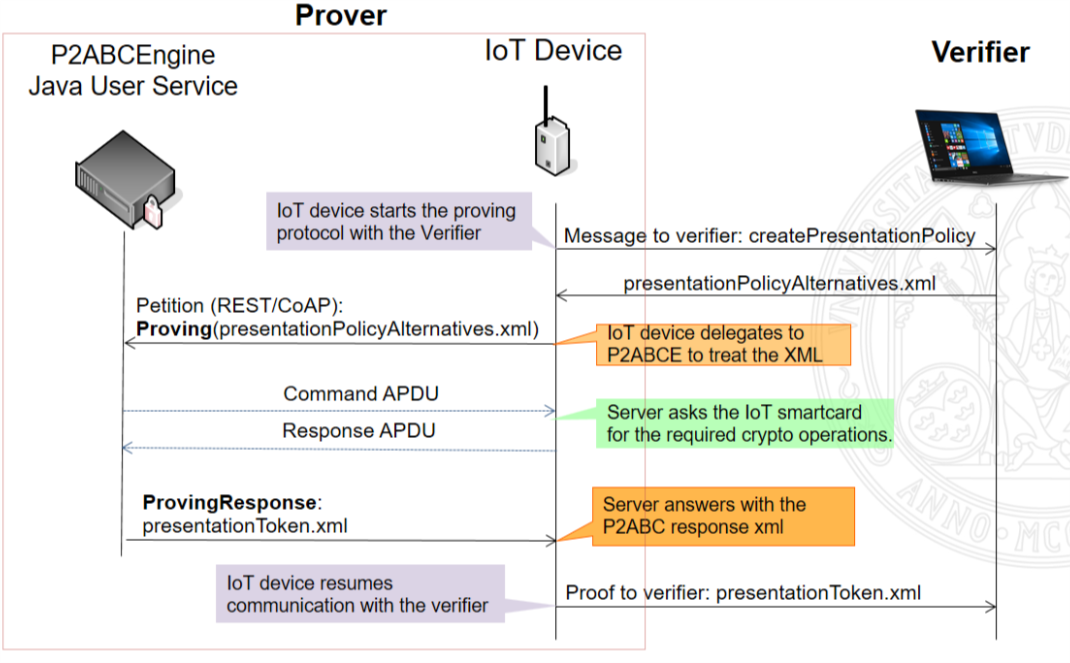
\includegraphics[width=\linewidth]{gfx/DelegationProving}
	\end{center}
	\caption{IoT Delegation in P2ABCE for Proving.}
	\label{fig:DelegationProving}
\end{figure}


\hfil


This simple design keeps the benefit of a 100\% compatible P2ABCE deployment, and the integration of IoT devices to the P2ABCE ecosystem.

In the future, more functionality currently delegated in the P2ABCE server can be implemented in the IoT device, if its resources allow it. For example, in a M2M environment, where an IoT device can act as User and Verifier, the verification consists on sending a Presentation Policy, and verifying the Presentation Token, which implies less logic than generating it as the User. Therefore, the implementation of the Verifier functionality would reduce significantly the need of a delegation server, but as we said, managing complex XML squemas is not something many IoT devices could do.




\section{IoT Smart Card}

After many design decisions in the process to adapt the original ABC4T Card Lite code to pure C, working over a more usual architecture machine, in this section, we present the current \ac{PoC} code, most important decisions, workflow execution, and future work.

First, let's define what a \textit{more usual architecture} is. If we remember the MULTOS section, the framework gives an application a very specific memory layout and entry and output points of execution, that could be seen as a single process execution machine. Many IoT devices work like a computer, with multiple processes or threads, without pre-loaded data on startup (like the APDU MULTOS loads for the application), a non-volatile memory for data and code, maybe a basic file system in this memory, and RAM with the program's stack, heap, data and code.

Our PoC is tested on a Linux system, and we will give instructions on how to adapt each part to work with other typical IoT systems.
For example, other IoT devices may work like MULTOS and let access variables in non-volatile memory during execution, and in that case, the port should be changed according to these particularities.


\hfil

\begin{figure}[bth]
	\begin{center}
		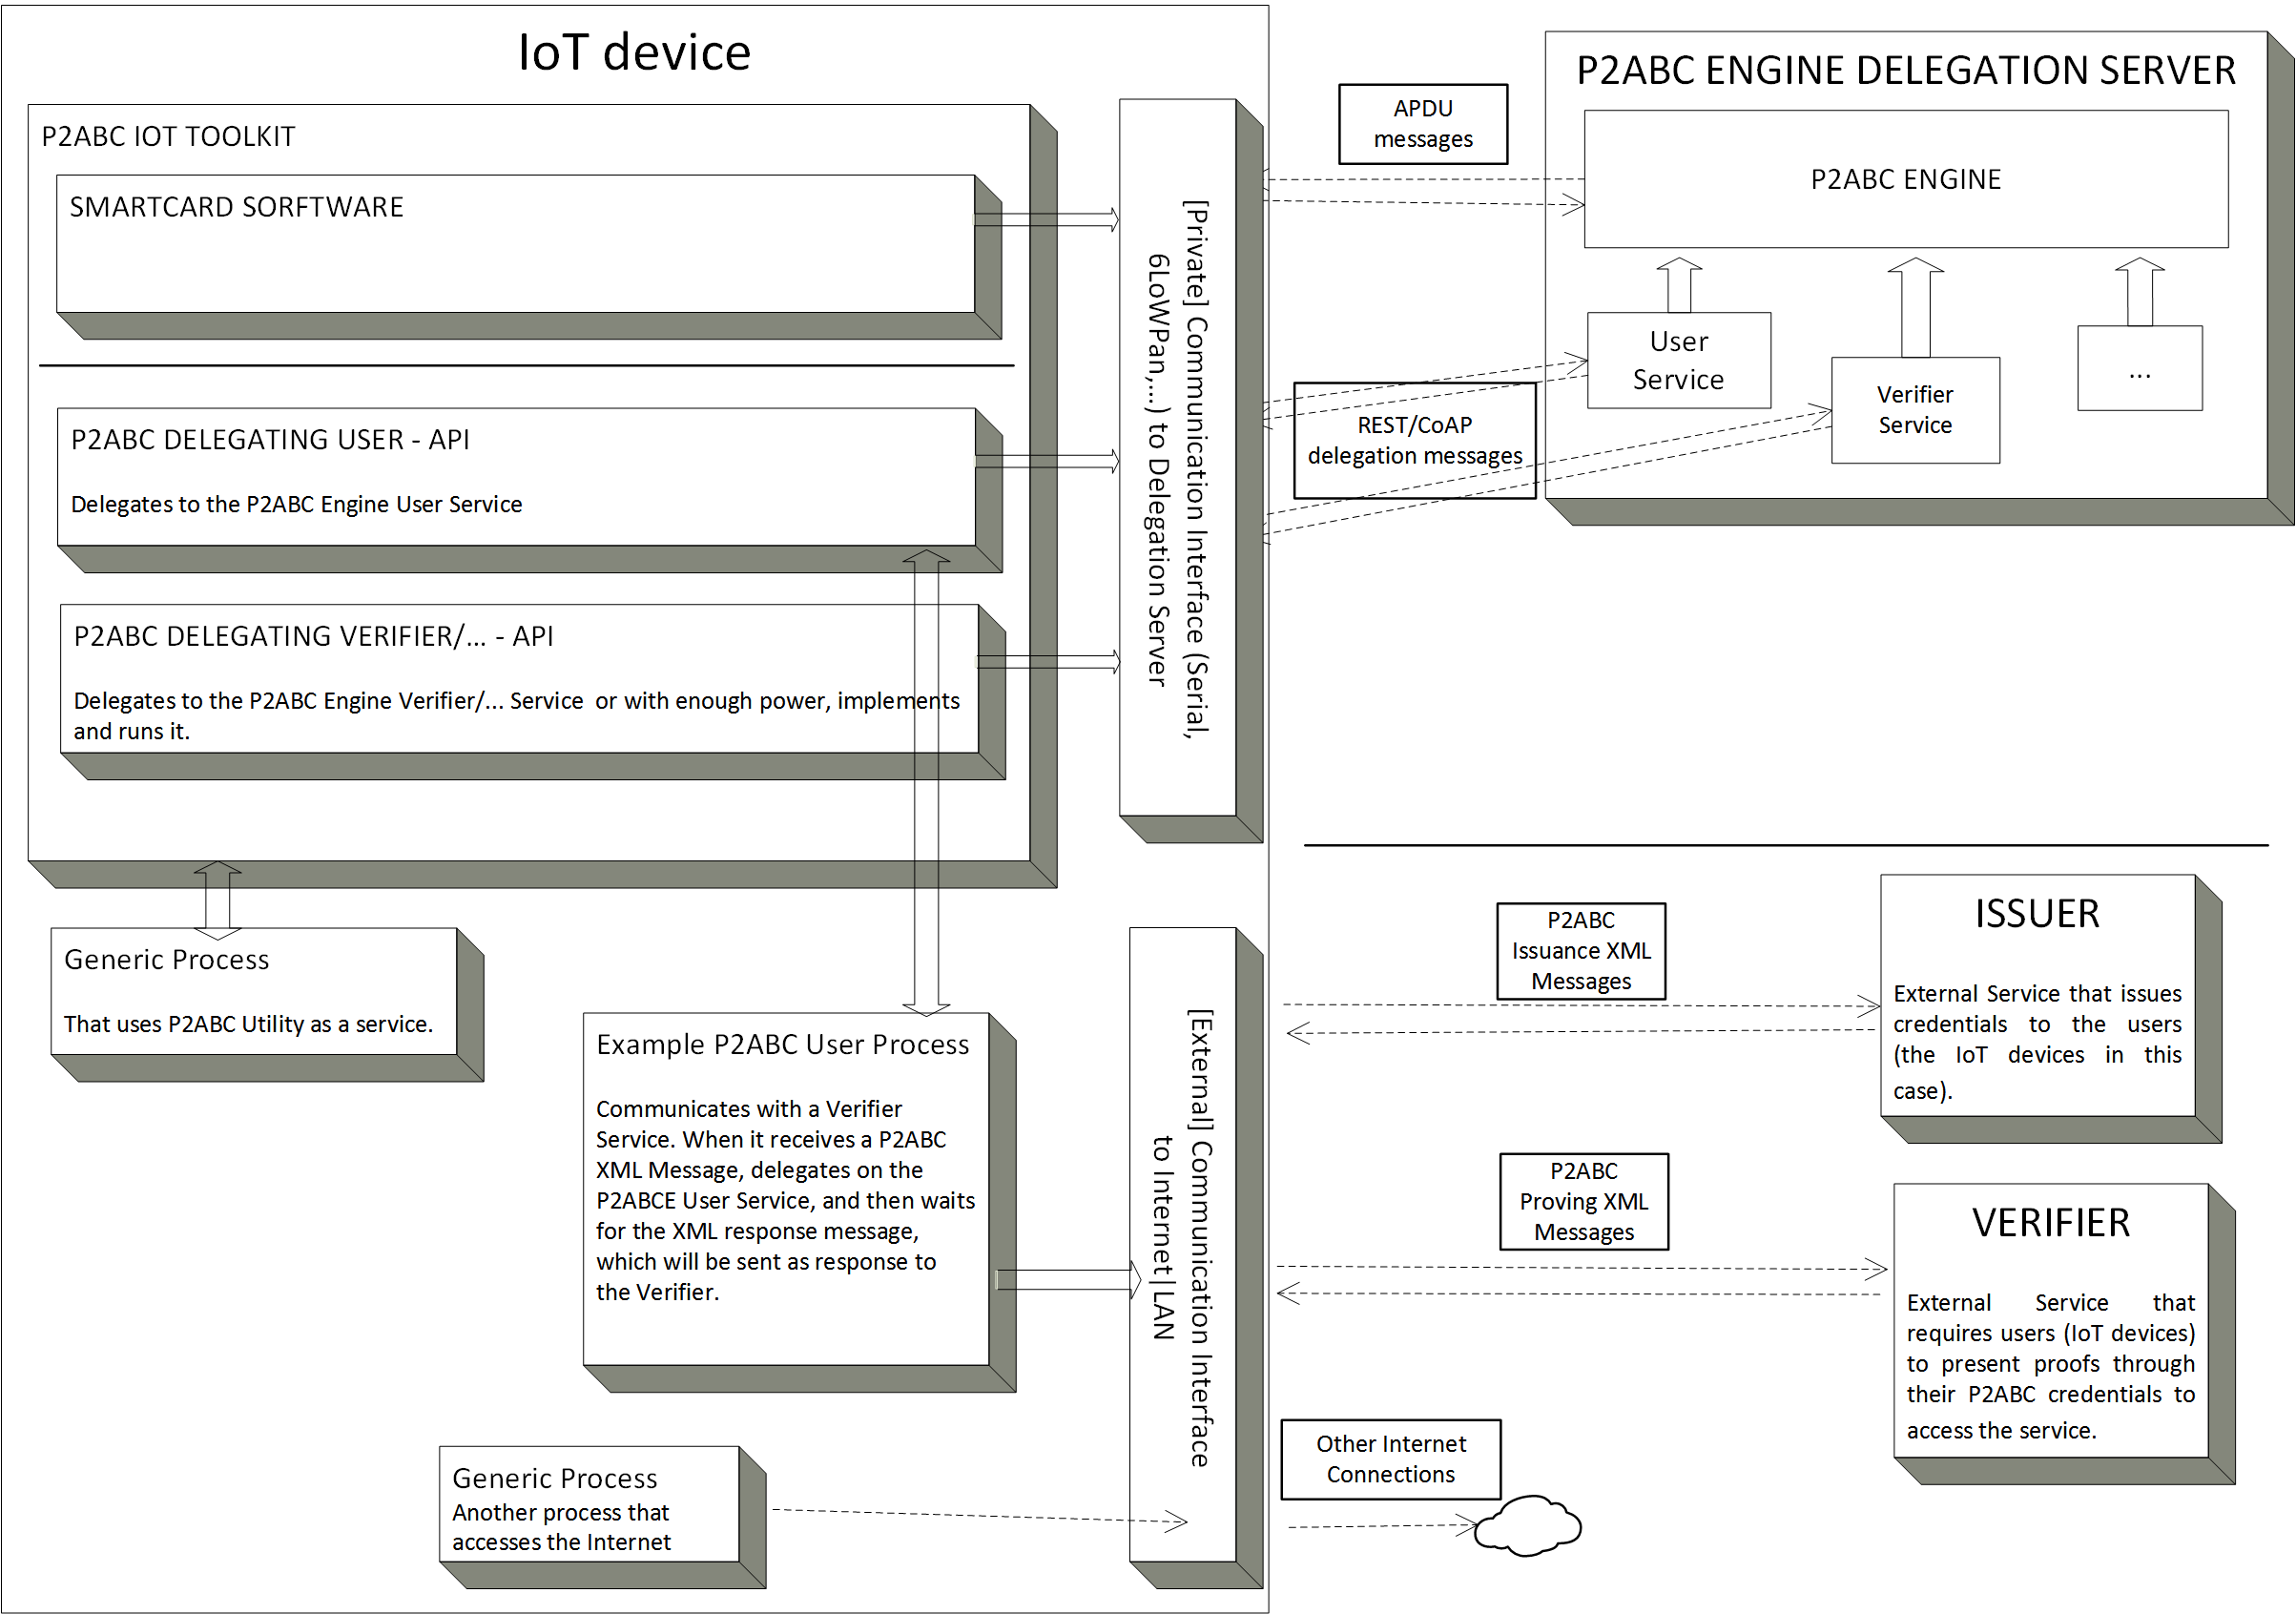
\includegraphics[width=\linewidth]{gfx/P2ABCE-IoT-bw}
	\end{center}
	\caption{IoT in P2ABCE deployment diagram.}
	\label{fig:P2ABCE-IoT}
\end{figure}

\begin{figure}[bth]
	\begin{center}
		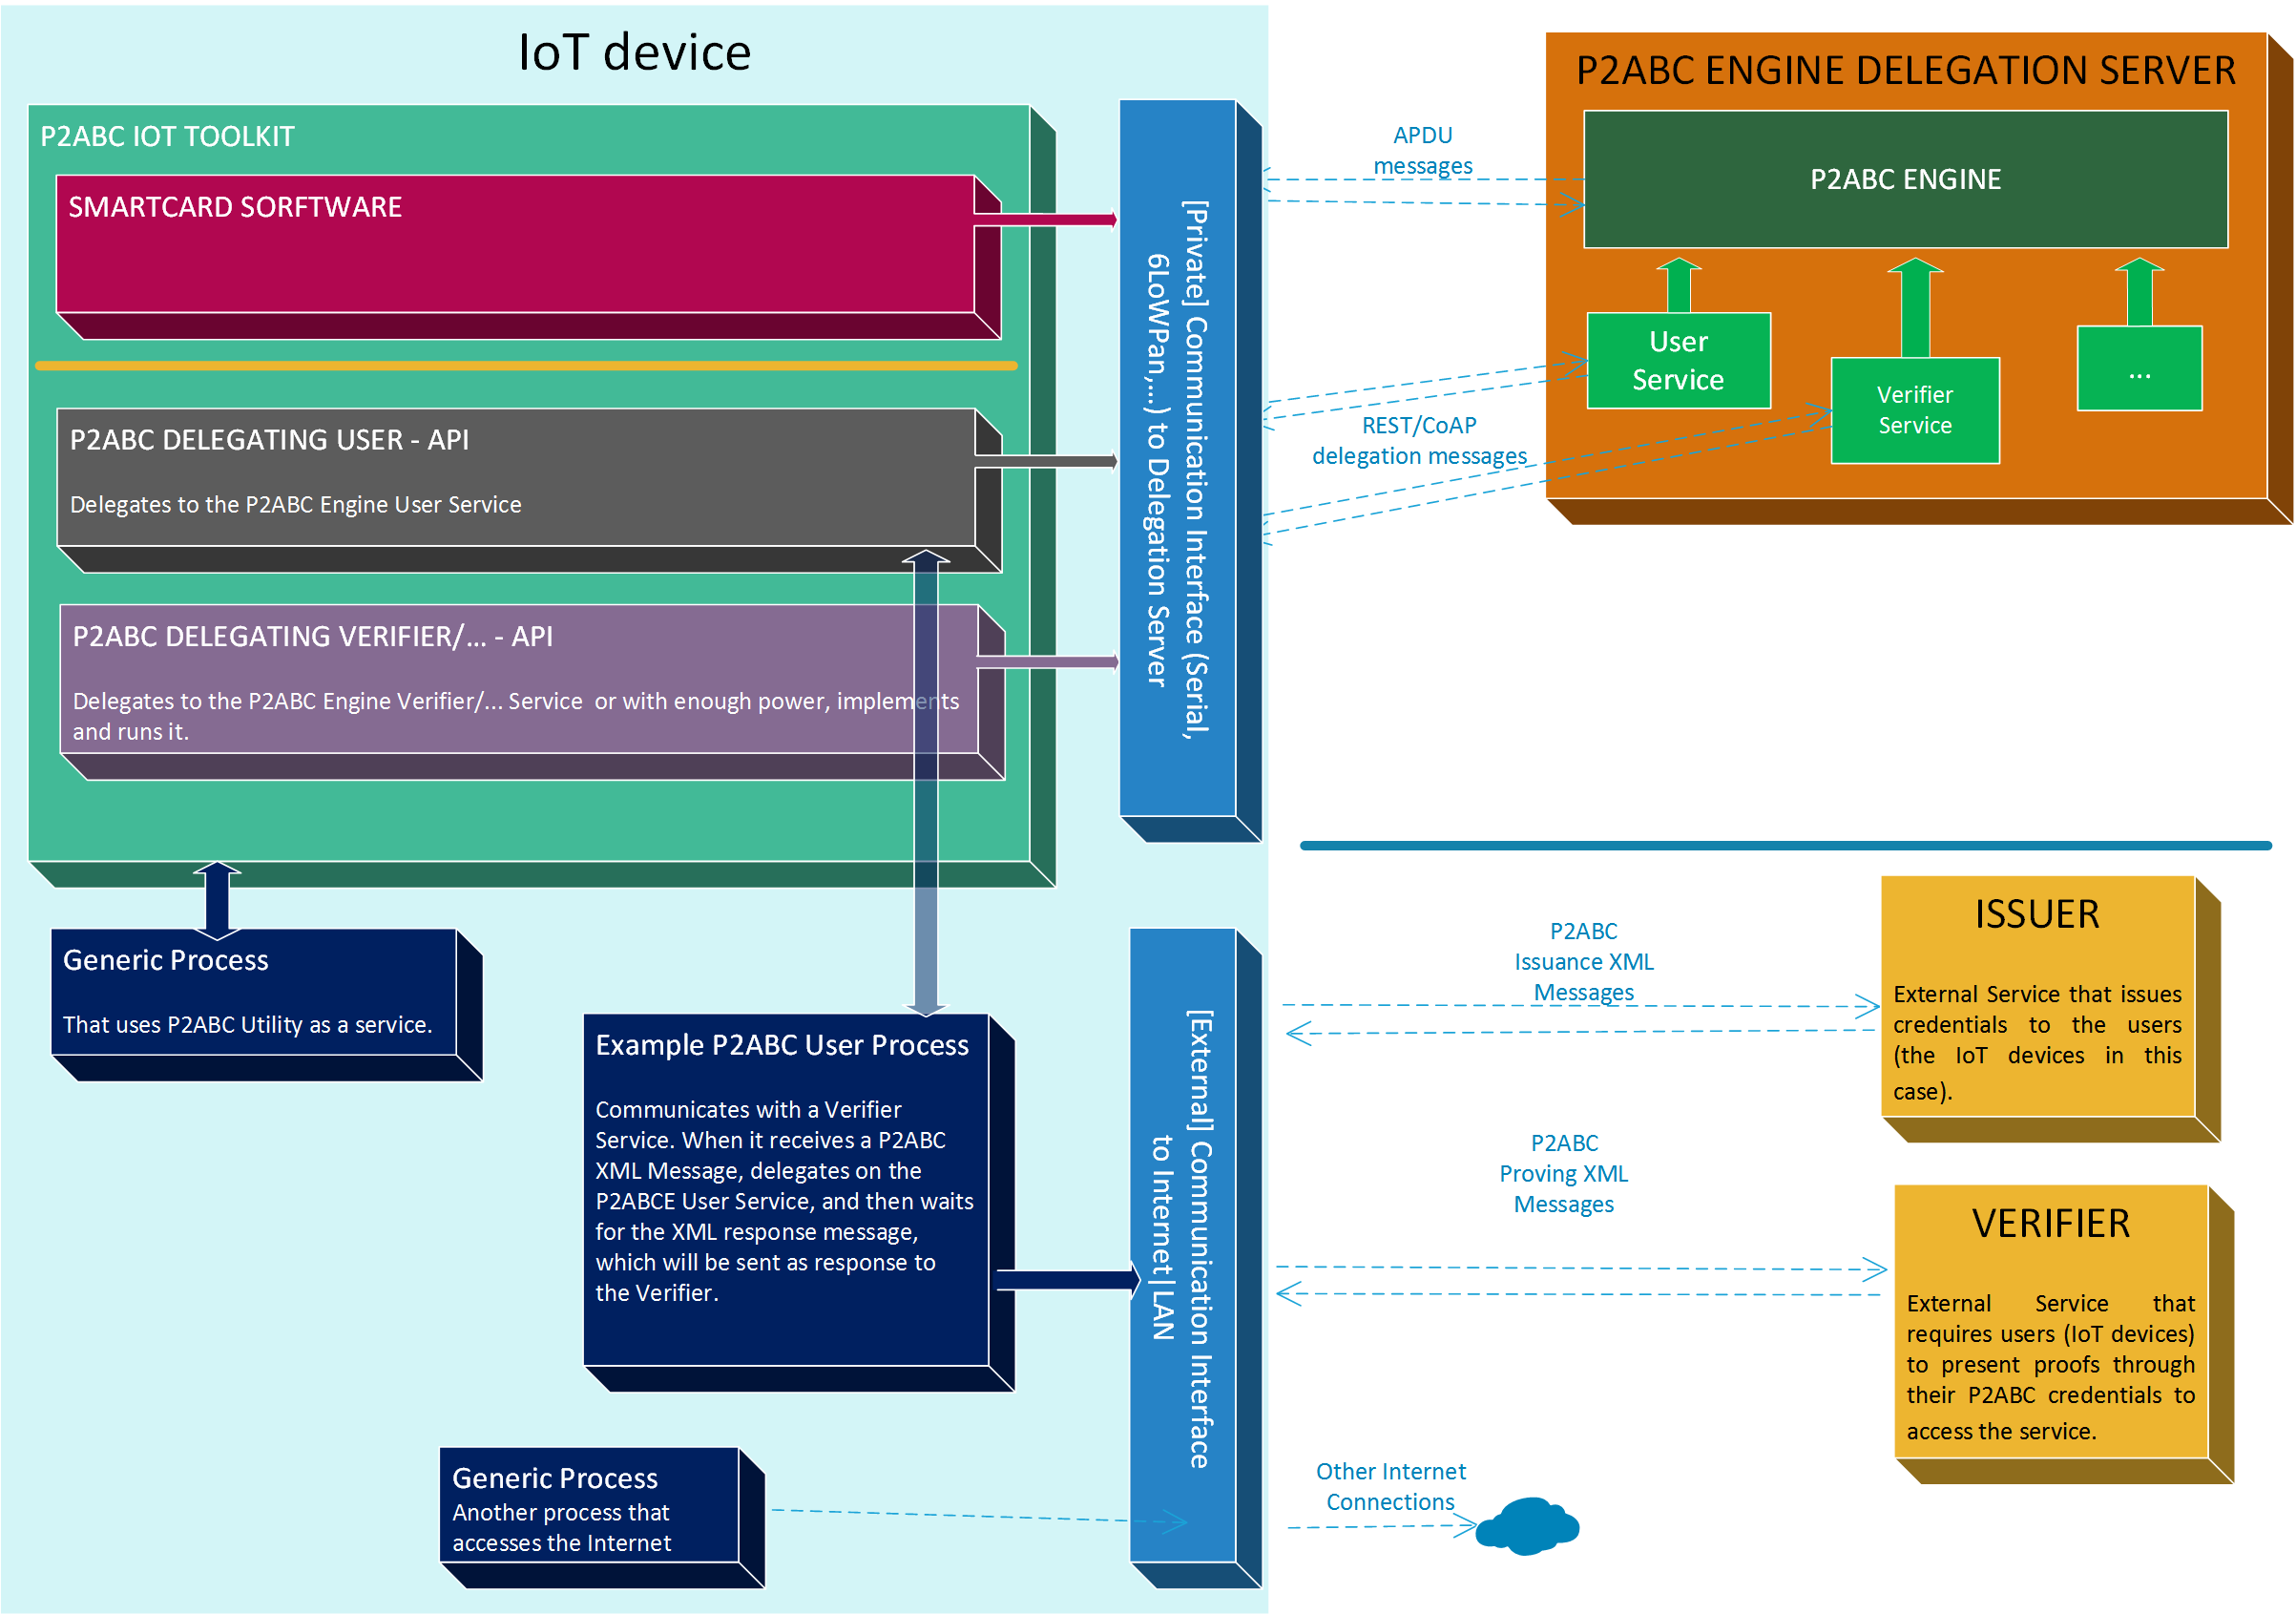
\includegraphics[width=\linewidth]{gfx/P2ABCE-IoT-color}
	\end{center}
	\caption{IoT in P2ABCE deployment diagram.}
	\label{fig:P2ABCE-IoT-color}
\end{figure}



\subsection{Code structure}


We divide the project in three different sections with the objective of enhancing maintainability, improving future changes, ports, fixes, etc.

The first section is what could be called as the core of the smart card, the second one the interface for the tools the core need and may depend on the platform, and finally third party libraries, that in may be empty if the interfaces implementation doesn't need any.


In our PoC we used CMake to manage the project, due to the cross-compilation tools, integration with multiple IDEs and tests.


\begin{figure}[bth]
	\begin{center}
		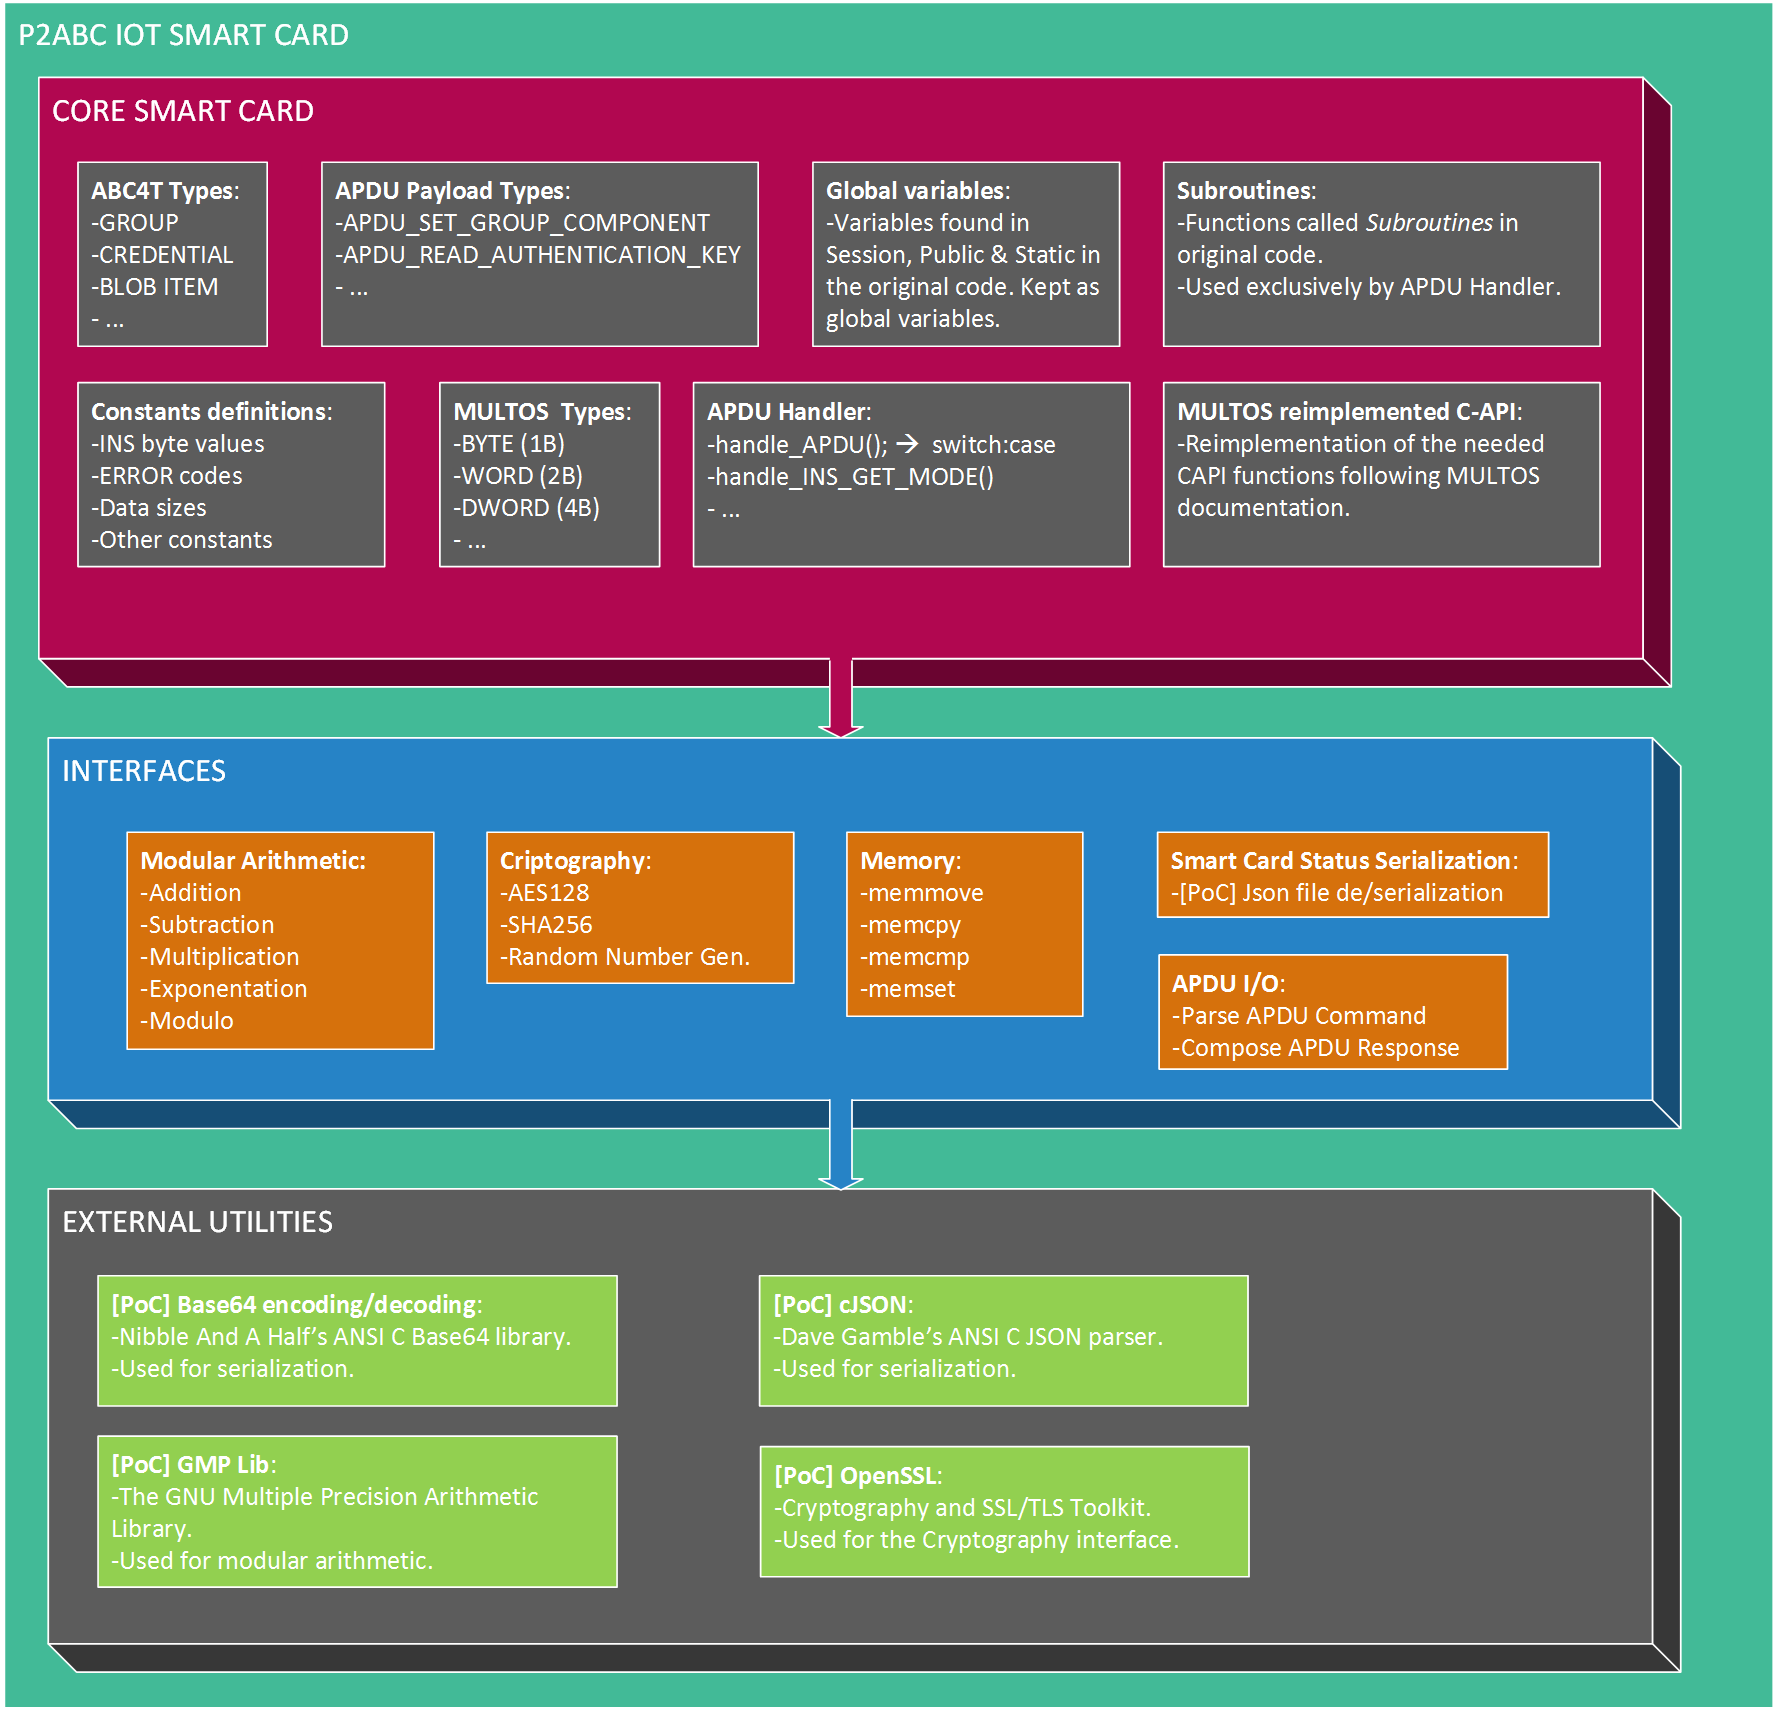
\includegraphics[width=\linewidth]{gfx/IoTCScomponents-color}
	\end{center}
	\caption{IoT Smart Card Code Structure.}
	\label{fig:IoTCScomponents-color}
\end{figure}

\begin{figure}[bth]
	\begin{center}
		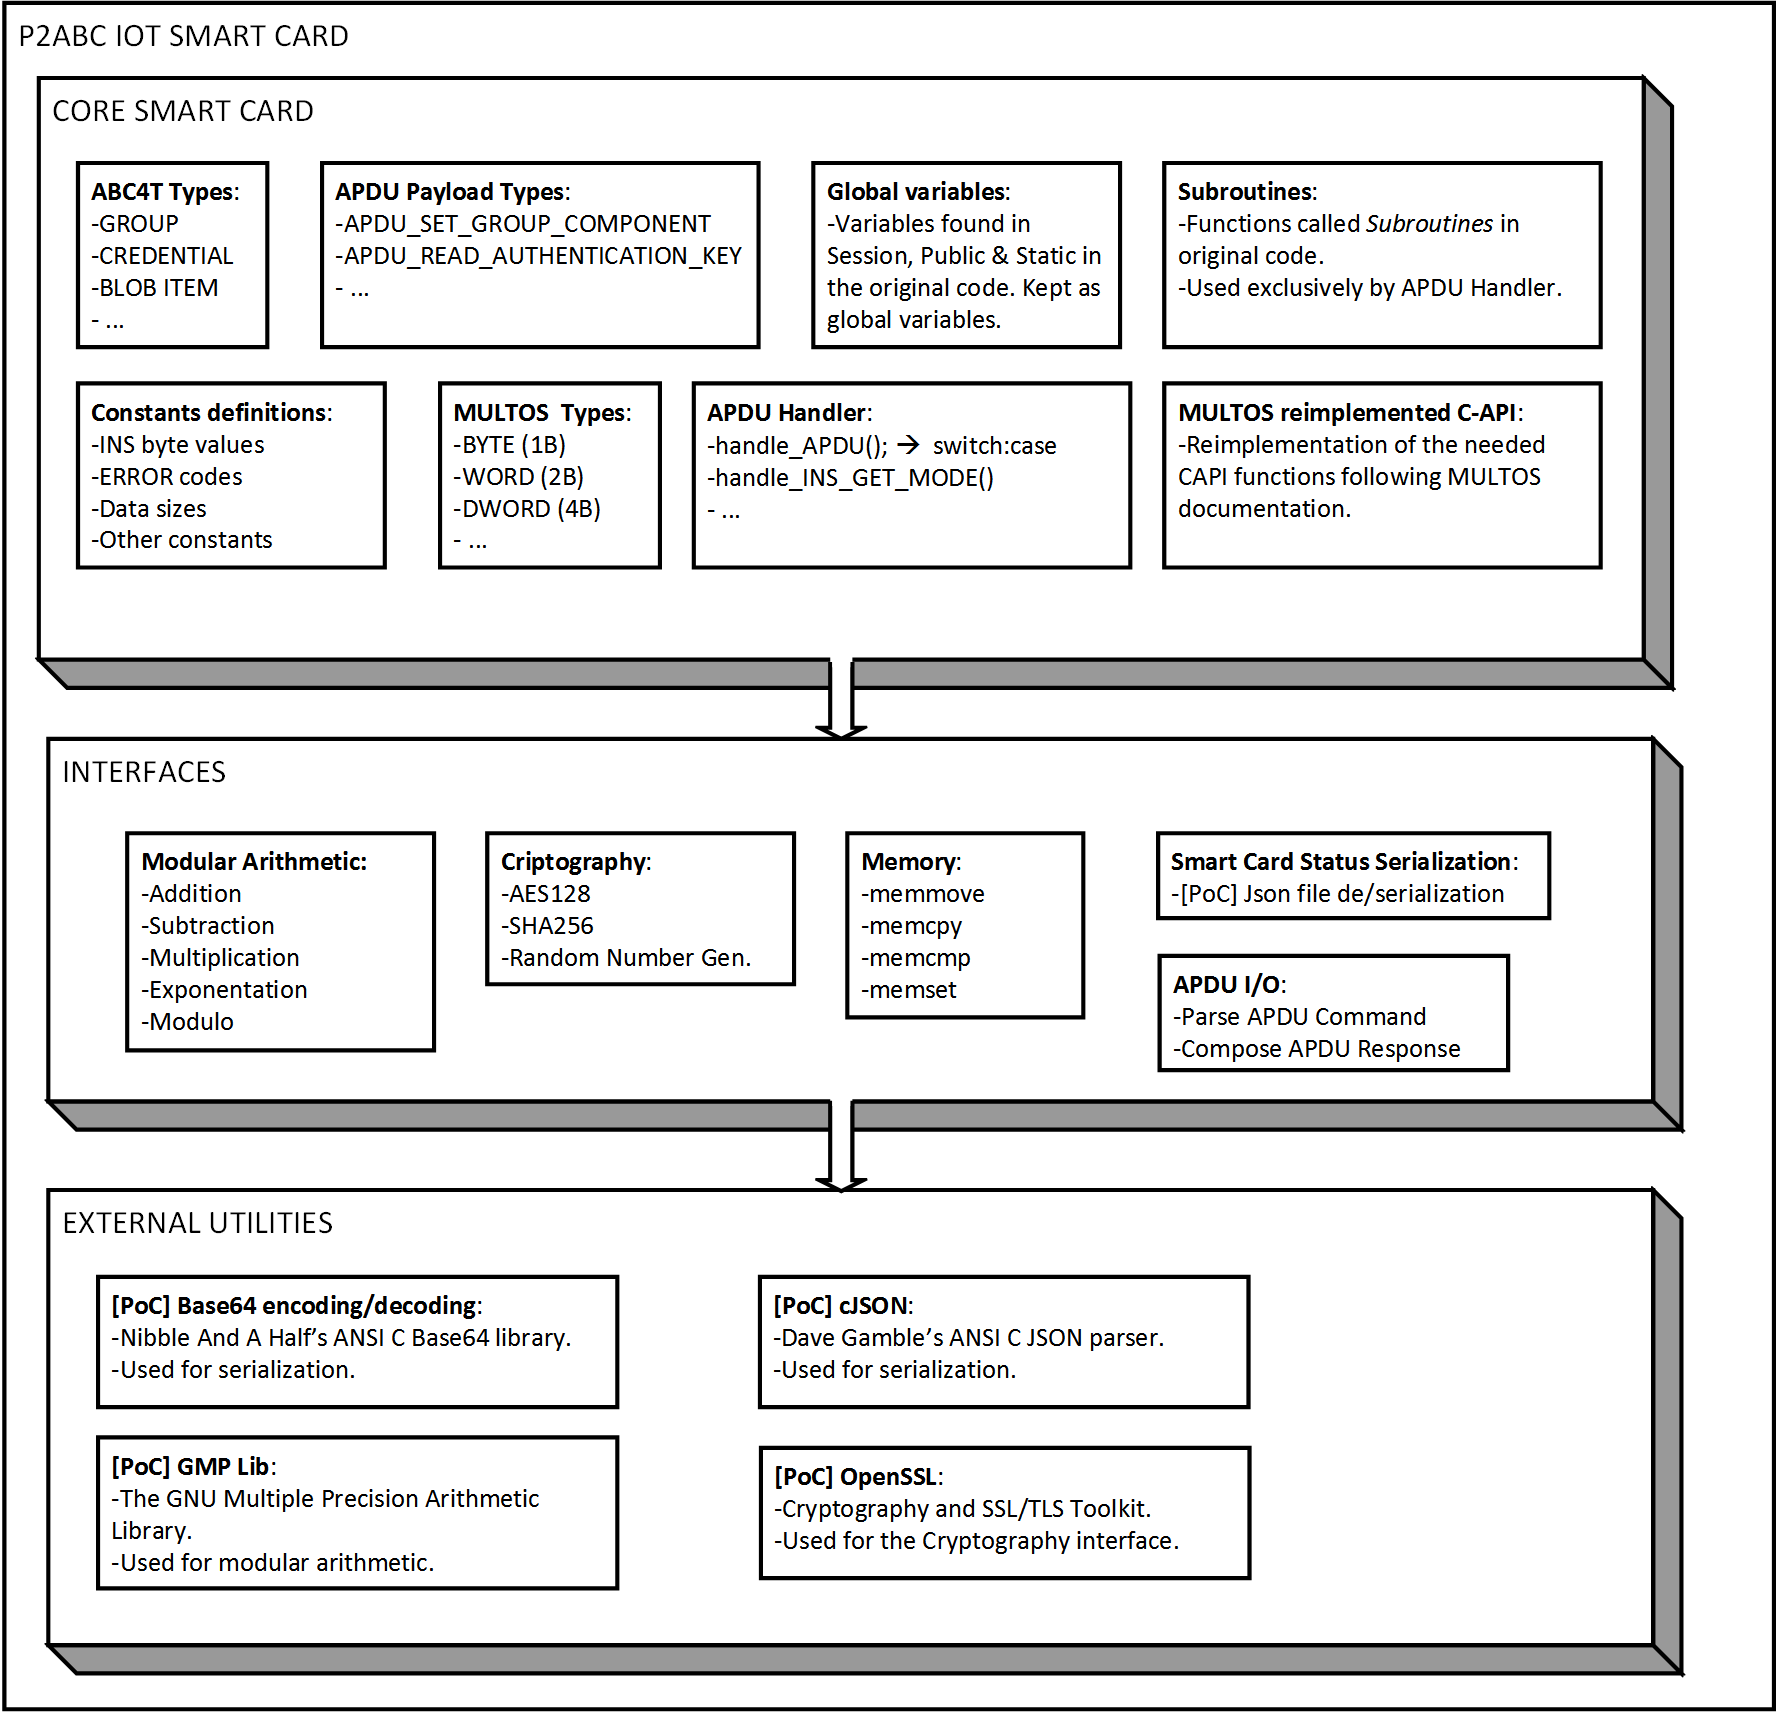
\includegraphics[width=\linewidth]{gfx/IoTCScomponents-bw}
	\end{center}
	\caption{IoT Smart Card Code Structure.}
	\label{fig:IoTCScomponents-bw}
\end{figure}


\hfil

\paragraph{Core smart card}

The smart card logic lies in this section, the concepts of APDU Commands, what instructions are defined in P2ABCE smart cards and how to process them and generate proper APDU Responses.

Changes in the APDU protocol for P2ABCE must be done here, independently of the target platform.

After refactoring the original ABC4Trust Card's code, most of it fell in what we will call the core of the smart card.

All types and variable definitions and the APDU handling is done in this code.
However, the ABC4Trust's code depended on the MULTOS C-API for the input/output of data, modular arithmetic, and even AES128 and SHA256 cryptography.

A characteristic of MULTOS C-API is that every function name starts with \textit{multos}, but as we said, the \textit{main.h} file implemented equivalent functions to some available in \textit{multos.h}. Our first step was to replace the \textit{main.h} functions for the standard ones in the C-API. Then, we implemented, following the C-API documentation, the functions from \textit{multos.h} (only the used ones) changing their names from \textit{multosFoo()} to \textit{mFoo()} for readability and emphasize that they were no longer from MULTOS.

Future changes in the code may refactor it so there's no longer need for the MULTOS framework functions.


\paragraph{Interfaces}

To implement MULTOS functions, we needed to use some libraries, so we defined a facade to isolate the implementation of the core smart card from our different options, that could vary depending on the hardware or the system used by the IoT device.

The use of a facade lets us, for example, change the implementation of modular arithmetic with a hardware optimized version, or a future more lightweight library, or our very own software implementation using the same data types that the core uses, minimizing the data transformations needed.

Taking a step forward, we make the core smart card totally independent of any library, only on our interfaces. This means that typical C libraries, like the standard \textit{stdlib.h}, or  \textit{string.h} are also behind the facade, in case some IoT system doesn't support them. The main goal we go after with this decision is that future developers adapting the code to a specific platform need to make no change to the \textit{core smart card}'s code, only to the interfaces implementation.



\paragraph{External utilities}

If the IoT system offers well tested libraries that could aid in the interfaces implementation, or we simply found a pure C implementation for the task, these third party libraries belong to this section.

In our PoC, we use two ANSI C libraries, for base64 and JSON, and two shared libraries available in as packages in LEDE, GMPLib and OpenSSL. The last two libraries offer more functionality than we need, hence, it's desired in a production code to implement \textit{Modular Arithmetic} and \textit{Cryptography} interfaces with more lightweight alternatives.

For example, Atmel's ATAES132A \citep{ATAES132A}
\marginpar{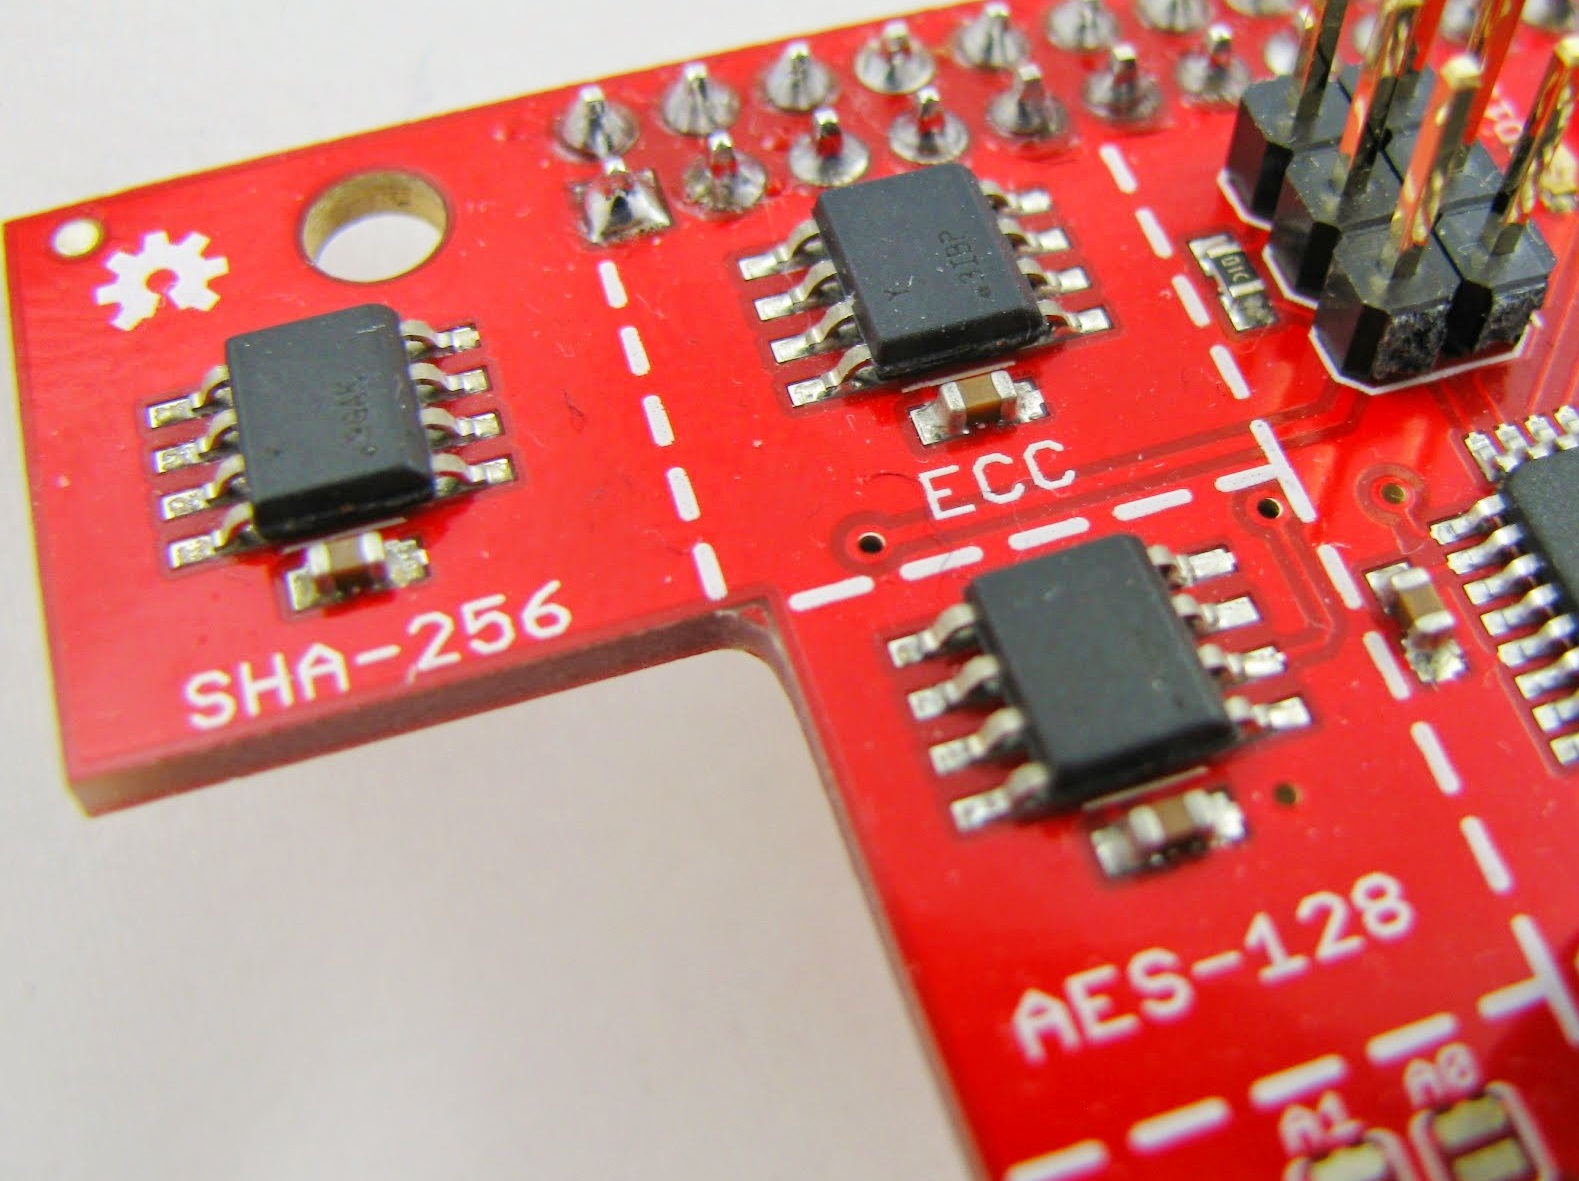
\includegraphics[width=\linewidth]{gfx/atmel} \\ Atmel's cryptography chips.}
offers a serial chip for secure key storage, AES128 execution and random number generation. Another serial chip like ESP8266 offers WiFi connectivity, typically used with Arduino, and can also perform AES encryption. For random number generation, a technique used with Contiki devices is to read from sensors aleatory data and use it as seed. All these alternatives depend on the target device, but are all valid. The \textit{interfaces} and \textit{external utilities} sections allow for a clean and fast port of the code.


\subsection{PoC Workflow}

% PoC BIOSC : TCP sockets, JSON serialization

% PoC IoT javax.smartcardio : protocolo de 2 bytes + APDU

% 1. Boot: deserialize sc status
% 2. Listening: open tcp socket
% 3. The IoT device delegates on the P2ABCE for some task and sends the IP and Port of the IoT Smart Card.
% 4. An APDU Command arrives : read in 2 bytes the length of the apdu and 


In a real deployment, we would offer a full library with an API to other processes to delegate on the P2ABC Engine, that automatizes the listening and security, that we presented in the deployment diagram \textbf{TODO:ref-img} as the \textit{P2ABCE IoT Toolkit}.

But to test the IoT smart card, we use the \textit{curl} command for REST delegation calls and the BIOSC (Basic Input Output Smart Card) for APDU communication.

To transmit the APDU messages in our PoC we use a simple protocol, consisting in one first byte for the instruction: receive an APDU Command or close the connection. In the first case, then we read two header bytes with the length of the APDU Command or Response to receive, followed by those APDU bytes. The message is sent over TCP for a reliable transmission (concept of session, packet retransmission, reordering, etc.).

We lack of any security (authentication and authorization) that a real system should implement. It is vital to authenticate the delegation service, to authorize it to make APDU Commands, and the same with the IoT device, to prevent attacks. This belongs to \textit{usual} security, as we already said, and for that reason it's not in the PoC.

\paragraph{P2ABCE REST Delegation}


The only P2ABCE Service that needed to be modified was the User Service. We added the REST call

\begin{center}
	\textit{/initIoTsmartcard/{issuerParametersUid}?host=\&port=}
\end{center}

where we communicate the P2ABCE server that a IoT Smart Card is accessible via \textit{host} and \textit{port}. Then a new \textit{HardwareSmartcard} object is stored in the P2ABC Engine, but instead of the \textit{javax.smartcardio} Oracle's \textit{CardTerminal} implementation, we use our \textit{IoTsmartcardio} implementation for the \textit{HardwareSmartcard} constructor.

The rest of P2ABCE code is unchanged and will work as if a real smart card was in use. \textit{IoTsmartcardio} implementation will transmit the APDUs through the TCP socket with the format mentioned.


\hfil

Our test consists on the tutorial available in P2ABCE's repository. From the Omega2's terminal we run \textit{curl} commands to send REST petitions. For example:

\begin{verbatim}
$ curl -X POST --header 'Content-Type: text/xml'
  'http://localhost:9200/user/initIoTsmartcard/http%3A%2F%2
  Fticketcompany%2FMyFavoriteSoccerTeam%2Fissuance%3Aidemix
  ?host=192.168.3.1&port=8888'
\end{verbatim}

The IoT device will only manage XML as data files to exchange between the third party actor and the P2ABCE delegation service, without parsing them.

After a REST call to the User Service, the P2ABC Engine will talk to the IoT smart card process.

\paragraph{APDU transmission with BIOSC}

% TODO : diagrama del software

Before sending the REST message, the Omega2 must be listening in the specified port. At start up, BIOSC reads from a JSON file the status of the smart card (credentials in the BLOB, private keys, PIN and PUK codes, etc.), then opens the TCP socket and listens in a loop.

When the delegation server sends an APDU Command following the simple protocol, BIOSC stores in a byte array the APDU Command bytes and calls the \textit{handle\_APDU} function in \textit{Core Smart Card}.


The \textit{APDU\_handler} will parse the APDU bytes and check both CLA and INS bytes. For each possible INS the is a function that must always finish calling either \textit{mExit()} or \textit{output\_large\_data()}.

The \textit{mExit} function is the reimplementation of MULTOS C-API exit functionality, that finishes the application execution returning to the MULTOS OS, that will send the APDU Response bytes to the terminal. This led in the original ABC4Trust Card's code to some tricky situations. Imagine a function that ends with an if-else expression. Many times we save a line writing something like

\begin{verbatim}
if(condition)
    return a;
return b;
\end{verbatim}

instead of the complete

\begin{verbatim}
if(condition)
    return a;
else
    return b;
\end{verbatim}

This is a swift example of what the \textit{multosExit} function led to, because it is called in both the \textit{switch-case} processing the APDU instruction, and the \textit{Subroutines}. For example, the PIN code check was programmed in a way every reason to fail finished the application execution, with different error codes. Another example, checking if a credential is stored, if not, fail and exit inside the \textit{readBlob} subroutine.

In our standard architecture machine, if we call a subroutine, it must end, and return the control to the handling function, and so the \textit{APDU\_handler} must return to the listening loop of BIOSC.

Having all that in count, the \textit{mExit} function is not implemented as the documentation specifies, but only saves the smart card status serializing it in the JSON file again, and once it's saved, parses the APDU Response and sends it to the socket.

The \textit{output\_large\_data} function is a tool used in MULTOS smart cards that don't support Extended APDUs. The APDU Command handler saves in a buffer the data to send, and its size. Then, \textit{output\_large\_data} will manage the buffer expecting future GET RESPONSE commands from the P2ABCE server.

A future change to the project may include support for Extended APDUs, avoiding the use of multiple GET RESPONSE. To do this, the \textit{output\_large\_data} function and the \textit{IoTsmartcardio} implementation of \textit{javax.smartcardio} must support the feature.

